\documentclass[10pt, conference, letterpaper]{IEEEtran}
\usepackage{cite}
\usepackage{xcolor,soul,framed}
\usepackage{amsmath,amsthm,amssymb,amsfonts}
\usepackage{algorithmic}
\usepackage{graphicx}
\usepackage{color, soul}
\usepackage{algorithm, algorithmic}
\usepackage[utf8]{inputenc}
\usepackage[english]{babel}
\usepackage{mathtools}
\graphicspath{ {./images/} }

%---------------------------------------------------------------%
\newtheorem{definition}{Denifition}
\newtheorem{assumption}{Assumption}
\newtheorem{problem}{Problem}
\newtheorem{lemma}{Lemma}
\newtheorem{corollary}{Corollary}
\newtheorem{example}{Example}
\newcommand{\eq}{=}
\newcommand{\domZ}{\mathbb{Z}_{*}}
\newcommand{\vecOne}{\mathbf{1}}
\newcommand{\ind}{\mathbf{I}}
\newcommand{\mat}{\mathbf}
\renewcommand{\vec}{\mathbf}
\DeclarePairedDelimiter\set\{\}
%---------------------------------------------------------------%
\newcommand{\apSet}{\mathcal{K}}
\newcommand{\esSet}{\mathcal{M}}
\newcommand{\jSet}{\mathcal{J}}
\newcommand{\wSet}{\mathcal{W}}
\newcommand{\uSet}{\mathcal{U}}
\newcommand{\cSet}{\mathcal{C}}
\newcommand{\Stat}{\mathbf{S}}
\newcommand{\Obsv}{\mathcal{O}}
%---------------------------------------------------------------%

\begin{document}

    %=============================== TITLE ===============================%
    \title{
        Meet-in-Future: Distributed Online Job Dispatching with Obsolete Information in Edge Computing System
    }
    \author{
        \IEEEauthorblockN{Yuncong Hong$^{*\dagger}$, Rui Wang$^{*}$, Haisheng Tan$^{\ddagger}$, Francis C.M. Lau$^{\dagger}$}
        \IEEEauthorblockA{
            $*$Southern University of Science and Technology, P.R. China,
            $\dagger$The University of Hong Kong, Hong Kong,\\
            $\ddagger$University of Science and Technology of China, P.R. China
        }
    }
    \maketitle

    %============================== ABSTRACT ==============================%
    \begin{abstract}
        \label{sec:abstract}
        Edge computing is believed to be the solid solution for time-sensitive big data real-time calculation. The cooperation among edge servers in the same coalition usually causes ineffective task scheduling due to obsolete information sharing, which is hard to tackle even with extra centralized agent design. In this work, we formulate the problem with job dispatching in distributed Edge Computing system, and identify the difficulty exists in cooperation between APs (Access Points) and ESs (Edge Servers) with delayed information. We design the broadcast information in the system and formulate the corresponding problem into a MDP problem. The value function approximation and \st{one-step policy iteration method is adopted to obtain a sub-optimal dispatching policy whose performance can be bounded analytically}.
    \end{abstract}

    % \begin{IEEEkeywords}
    %     Edge Computing, Job Dispatch, Delayed Information, Collective Observability, Distributed Multi-agent MDP
    % \end{IEEEkeywords}

    %============================ INTRODUCTION ============================%
    \begin{section}{INTRODUCTION}
        \label{sec:introduction}
        Our claims:
        \begin{itemize}
            \item Related works on scheduling in edge computing, mostly with centralized agent to apply action and seldomly take delayed information impact into consideration;
            \item Edge Server, Access Point, User Equipment; layered structure where decision is made distributedly on APs and computation is carried out on ESs; The AP-ES fully connected structure is reasonable, for example C-RAN to separate communication and computation 
            \item We identify the delayed system information is un-acceptable for explosion \emph{delay-sensitive jobs} in edge computing, and it's hard to establish cooperation among APs because of obsolete information;
            \item information sharing for cooperation is designed via (aligned) broadcast, job dispatch decision should be made immediately based on the previous collective information;
        \end{itemize}

        Our contributions:
        \begin{itemize}
            \item identify a instant job dispatch fully-distributed cooperative way, and avoid the centralized agent design;
            \item identify the uploading process may affect the heuristic greedy algorithm performance; identify the delay-information affected decision making;
            \item propose a global consensus state method to formulate the MDP problem (we use MDP definition in \cite{sutton1998introduction});
            \item adopt value function approximation to reduce the traditional algorithm complexity, and come up with distributed online learning algorithm;
        \end{itemize}

        Related works:
        \begin{itemize}
            \item The earliest related works we find is \cite{ref-01} (cited 167 times). In this work, the single agent is assumed not able to observe the global state, and thus they need communication to establish cooperation by sharing \emph{information}. The agent considers communication as extra action to synchronize the states and thus incurs extra cost. \\
            However, the communication is without delay, and converted into POMDP problem.
            \item The other work \cite{ref-02} considers continuous state observation with constant or stochastic delay with single agent. \\
            However, 
        \end{itemize}

    \end{section}

    %============================ SYSTEM MODEL ============================%
    \begin{section}{SYSTEM MODEL}
        \label{sec:model}
        \begin{subsection}{Network Model}
            The network topology of the MEC system considered is illustrated in Fig. \ref{fig:system}, which is composed of three elements. The user equipment (UE) is connected to access point (AP) and . The AP provides network access to all the UEs connected and also fully connected with each other to share nodes' information. The AP itself is assumed with no computation capability, and then dispatch the jobs from UEs to backend edge servers (ES) in a distributed cooperative way. Moreover, the network topology between AP cluster and ES cluster is also assumed fully connected for the reason that they are in the same coalition.
            \begin{figure}[ht]
                \centering
                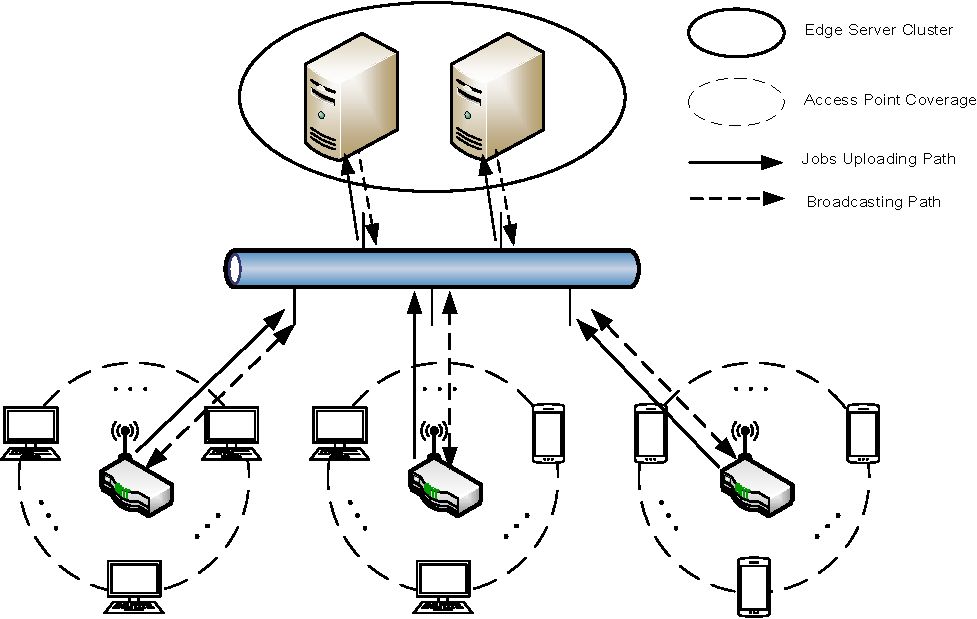
\includegraphics[width=0.45\textwidth, trim={0.5cm 0.5cm 0.5cm 0.5cm}, clip]{system-model.pdf}
                \caption{The Illustration of MEC System Model}
                \label{fig:system}
            \end{figure}

            Let $\mathcal{K} \triangleq \set{1,\dots,K}$ and $\mathcal{M} \triangleq \set{1,\dots,M}$ denote the set of APs and set of ESs in the MEC system respectively. We adopt \emph{timeslot} lasting for $\tau$ seconds as the minimum time slice in the system, and the dispatching and scheduling decision on AP and ES side respectively are all applied based on this timing. Furthermore, we assume the job arrival process for AP nodes is illustrated as follow:
            \begin{assumption}
                (Job Arrival Process at AP).
                We assume that the job arrival process $A_k(t)$ for $k$-th AP is i.i.d over the timeslots and each with Bernoulli distribution as $A_k(t) \sim Bernoulli(\lambda_k)$.  According to Poisson Limit Theorem, we identify the arrival process as memory-less exponential process and with average arrival rate as $\mathbb{E}[A_k(t)] = \lambda_k$.
                This assumption implies that there will be at most one job arrives AP in one timeslot from all the UEs connected.
            \end{assumption}

            There are two main communication process with APs and ESs engaged based on the network topology elaborated above. We assume the communication latency is rather deterministic between two nodes and assign the delay time directly w.r.t transmission content for convenience.

            The first one is \emph{uploading process} where AP dispatches jobs to corresponding ESs. The uploading time for all kinds of jobs is same for one AP-ES link, as $T^{prop}_{k,m}$ from $k$-th AP to $m$-th ES where $T^{prop}_{k,m}$ will always last for integer timeslots. \emph{Parallel uploading} is enabled on AP to alleviate the cost caused by serially uploading process; as the arrival process and uploading time is bounded, there will be at most $\lambda_k \cdot \max_m(T^{prop}_{k,m})$ jobs in transmission on $k$-th AP which results into finite bandwidth requirement.
            
            The other one is \emph{broadcast process} to facilitate cooperative dispatching decision.
            The information sharing among distributed AP nodes is designed via broadcast to achieve global optimality. The AP nodes should broadcast their system information to the other AP nodes, and the ES nodes should broadcast their information to all the AP nodes. More specifically, all the APs and ESs start to broadcast at the same start point at the beginning of one time slot and repeat broadcasting with the same interval as $T_{br}$ timeslots, which is called \emph{aligned broadcast}. Let $d_{k,i}$ denotes the broadcast delay from $i$-th node ($i\in\apSet$ or $i\in\esSet$) to $k$-th AP w.r.t to the last broadcast point where $d_{k,k} \equiv 0$ for convenience, and the broadcast interval is always larger than the broadcast delay, i.e. $T_{br} > d_{k,i}$.
            Furthermore, we elaborate the concept called \emph{consensus delay} for AP nodes as:
            \begin{definition}
                (Consensus Delay).
                \begin{align}
                    \hat{d}_k = \max_{j\in(\apSet\cup\esSet)}(d_{k,j})
                \end{align}
                where $d_{k,k} \equiv 0$; the consensus delay for $k$-th AP is the delay after the last broadcast point where it could update the global information consensus.
            \end{definition}
            The aligned broadcast is guaranteed by timely synchronization protocol and is not the main component in our discussion. \st{The details of  broadcast information will be elaborated in the following section \emph{Job Dispatch Model}.}
        \end{subsection}

        \begin{subsection}{Computation Model}
            For computation process on edge servers, we adopt \emph{unrelated machines} assumption in \cite{tan-online}, where the job processing time on different servers are machine dependent and variant of resource or VM (virtual machine) constraints. The processing time is with upper bound as $L_C$, and the job set is denoted as $\mathcal{J} = \set{0,1,\dots, J}$ where $J=L_C^M-1$ for all possible length combination; the $j$-th job in $\jSet$ has the computation time as $\vec{l}_j = ([l_j^1, l_j^2, \dots, l_j^M] + \vecOne^M)$ on edge servers cluster $\esSet$, where $\vec{l}_j$ is the index $j$ under $L_C$-base denotation. Additionally, we denote PDF of the release distribution over $\jSet$ as $\Pr(\jSet)$.
            We assume the scheduling policy on all the servers are identical as following:
            \begin{assumption}
                (Scheduling Policy).
                \hl{(could be removed if we stress both dispatching and scheduling optimization, i.e. SJF job scheduling)}
                All the edge servers adopt \emph{FCFS} (First-Come-First-Serve) as job scheduling policy, i.e. the job earlier arrives at the server would get served earlier. And we note that the arrival order is not only determined by job arrives at the access point, but also related with the uploading latency.
            \end{assumption}
        \end{subsection}

        \begin{subsection}{Job Dispatching Model}
            The lifetime of jobs dispatching is composed of three stages: waiting on APs for uploading, in uploading to servers, and waiting for service on servers queue. The three stages results into jobs set accumulation on APs and ESs which is illustrated in Fig. \ref{fig:trans}, and the Markovian transition relationship between the adjacent timeslot.

            The local states on APs and ESs are divided into three job set:
            \begin{itemize}
                \item Let $\wSet_{k}(t)$ denotes the job set on $k$-th AP $\forall k \in \apSet$, which comprises the jobs waiting for dispatching decision at $t$-th timeslot; $w \triangleq (\vec{l}_i) \in \wSet_{k}(t)$, where $w$ denotes the tuple containing one element $\vec{l}_w \in \domZ^M$ as the computing length on all $M$ unrelated edge servers.
                \item Let $\uSet_{k,m}(t)$ denotes the jobs in uploading from $k$-th AP to $m$-th ES in $t$-th timeslot $\forall k \in \apSet, m \in \esSet$; $u \triangleq (l_u, T_{u}(t)) \in \uSet_{k,m}(t)$, $l_u$ denotes the computing length on $m$-th server and $T_{u}(t)$ records the remaining time for uploading completed.
                \item Let $\cSet_{m}(t)$ denotes the jobs waiting for computing on $m$-th ES in $t$-th timeslot; $c \triangleq (t_c, T_{c}(t)) \in \cSet_{m}(t)$; $t_c$ denotes for arriving timestamp at server, $T_{c}(t)$ denotes for the remaining time for computing completed.
            \end{itemize}

            Then we have the denotation of system observation in $t$-th timeslots on left-hand side in the figure as:
            \begin{align}
                \mathcal{O}(t) \triangleq (\bigcup\limits_{k\in\apSet}\wSet_{k}(t), \bigcup\limits_{k\in\apSet, m\in\esSet}\uSet_{k,m}(t), \bigcup\limits_{m\in\esSet}\cSet_{m}(t))
            \end{align}
            and as the transition is initialized by \emph{dispatching decision} and therefore automatically been uploaded and computed, we give the definition for decision action here:
            \begin{definition}
                (Dispatching Action).
                The dispatching action is applied job-wise in the waiting job set denoted as $\vec{a}: j \to \set{0,1,\dots,M}, \forall j\in\jSet$, where $a_j\eq0$ means $j$-th job should keep waiting and $a_j=m\neq0$ means $j$-th job should be uploaded to $m$-th ES. The waiting decision is transient as the jobs are always been uploaded at last.
            \end{definition}

            Then we characterize the job dispatching process by Markovian transition between adjacent timeslots.
            We come up with denotations for transition job sets expressed in Fig. \ref{fig:trans} as:
            \begin{align}
                \wSet'_{k}(t) &\triangleq \wSet_{k}(t) \cup A_k(t)
                \\
                I^{(W \to W')}_{k}(t) & \triangleq \{ w | a^{(k)}(L_C^{\vec{l}_w})\eq0, \forall w \in \wSet'_{k}(t) \}
                \\
                I^{(W \to U)}_{k,m}(t) &\triangleq \{ w | a^{(k)}(L_C^{\vec{l}_w})=m, \forall w \in \wSet'_{k}(t) \}
                \\
                I^{(U \to C)}_{k,m}(t) &\triangleq \{ u | T_{cd,u}=1, \forall u \in \uSet_{k,m}(t)\}
                \\
                I^{(U \to U')}_{k,m}(t) &\triangleq \uSet_{k,m}(t) \backslash I^{(U \to C)}_{k,m}(t)
                \\
                I^{(C \to \Phi)}_{m}(t) &\triangleq \{ c | \arg\min_{c\in\cSet(t)} T_{cd,cc}(t) \wedge T_{cd,c}=1\}
                \\
                I^{(C \to C')}_{m}(t) &\triangleq \cSet_{m}(t) \backslash I^{(C \to \Phi)}_{m}(t)
            \end{align}
            where $I^{(W \to W')}_{k}(t), I^{(U \to U')}_{k,m}(t), I^{(C \to C')}_{m}(t)$ denote the job sets not engaged in transition, $I^{(W \to U)}_{k,m}(t), I^{(U \to C)}_{k,m}(t)$ denote the jobs beginning uploading and uploaded on server respectively, and $I^{(C \to \Phi)}_{m}(t)$ denotes the job that leaves from the system on $m$-th ES in $t$-th timeslot.
            Then we establish the relationship between those indicator functions with $\mathcal{O}(t+1)$ as:
            \begin{align}
                \begin{cases}
                    \wSet_{k}(t+1) = I^{(W \to W')}_{k}(t)
                    \\
                    \uSet_{k,m}(t+1) = I^{(W \to U)}_{k,m}(t) \cup I^{(U \to U')}_{k,m}(t)
                    \\
                    \cSet_{m}(t+1) = \bigcup\limits_{k\in\apSet} I^{(U \to C)}_{k,m}(t) \cup I^{(C \to C')}_{m}(t)
                \end{cases}
            \end{align}
            and we notice that no matter job arrival or decision on $\wSet$ happened or not, the attributes of jobs in $\uSet$ and $\cSet$ have to change according to the deterministic rule about uploading and scheduling respectively, which is not stated explicitly in the above transition cases.

            \begin{figure}[ht]
                \centering
                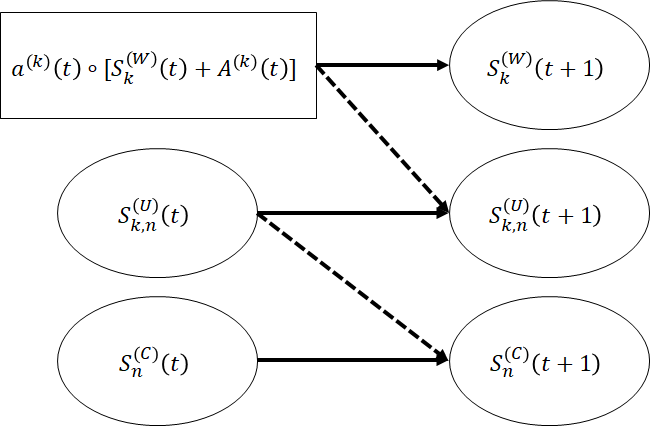
\includegraphics[width=0.42\textwidth]{single-transition.png}
                \caption{Single-step transition function composing graph}
                \label{fig:trans}
            \end{figure}

            Additionally, the broadcast design is not engaged in dispatching model for now but it will have affects on dispatching decision which will be illustrated in next section.
        \end{subsection}
    \end{section}

    %============================ FORMULATION =============================%
    \begin{section}{FORMULATION}
        \label{sec:formulation}
        In this section, we formulate the standard MDP problem based on the MEC system elaborated above. The optimization problem will be formulated globally on dispatching decisions on APs, but applied fully distributed on each AP with broadcast design to share information.

        \begin{subsection}{System State and Scheduling Policy}
            Before we give the canonical definition for system states in the distributed system, we firstly clarify the broadcast information from AP nodes and ES nodes. For convenience, we denote the broadcast point as $T_\tau$ where:
            \begin{align}
                T_\tau = \tau \cdot T_{br}, \tau=0,1,2\dots
            \end{align}
            furthermore, we denote the observation at broadcast point $T_\tau$ as $\Obsv_\tau$. The broadcast information is based on $\Obsv_\tau$ as:
            \begin{definition}(Broadcast Information).
                The $k$-th AP would broadcast all the job set information at $T_\tau$ as $\wSet_{k}(T_\tau), \bigcup\limits_{m\in\esSet}\uSet_{k,m}(T_\tau)$, and the accumulated number of jobs in last broadcast interval as:
                \begin{align}
                    n^{(k)}_\tau = \sum_{t=T_{\tau-1}}^{T_\tau-1} |\wSet_{k}(t)| + |\bigcup\limits_{m\in\esSet}\uSet_{k,m}(t)|,\forall k \in \apSet
                \end{align}
                \\
                The $m$-th ES would broadcast the job set information at $T_\tau$ as $\cSet_{m}(T_\tau)$ and also the accumulated number of jobs in last broadcast interval as:
                \begin{align}
                    n^{(m)}_\tau = \sum_{t=T_{\tau-1}}^{T_\tau-1} |\cSet_{m}(t)|,\forall m \in \esSet
                \end{align}
                \\
                We have the vector $\vec{n}_\tau$ to denote the accumulated number information from all the APs and ESs, and thus the composed broadcast information at $T_\tau$ is denoted as:
                \begin{align}
                    \tilde{\Obsv}_{\tau} = (\Obsv_\tau, \vec{n}_\tau)
                \end{align}
                and we have $\vec{n}_0 = \mathbf{0}$ with empty initialized system.
            \end{definition}

            This broadcast information is also called \emph{global consensus} in Fig. \ref{fig:br-trans} \hl{(need to modify the state denotation)} that $k$-th AP would only obtain the broadcast information completely after the \emph{consensus delay} $\hat{d}_{k}$ w.r.t to the last broadcast point. The system state of the formulated MDP problem is on the global consensus but locally computed at each AP nodes, given as follow:
            \begin{definition}(System State).
                The $\tau$-th state is: $\Stat_\tau = (\Obsv_{\tau}, \Obsv_{\tau-1}, \vec{n}_\tau)$, $\tau=1,2,\dots$ for all the AP nodes. Though the $k$-th AP nodes would come up with this state after $\hat{d}_k$ timeslots, it will accept the obsolete information and adopt actions for job dispatching on it.
            \end{definition}
            \begin{figure}[ht]
                \centering
                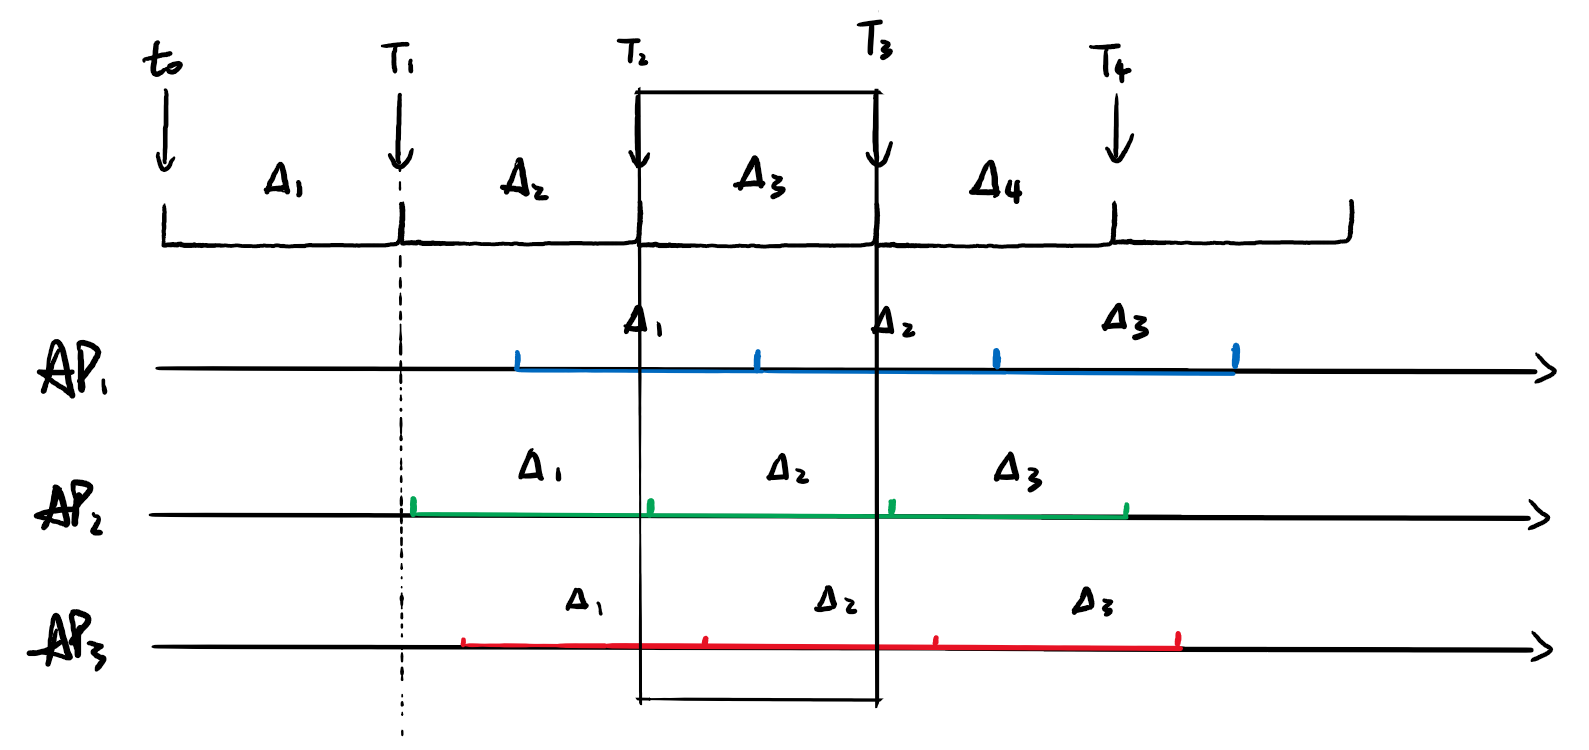
\includegraphics[width=0.45\textwidth]{broadcast-trans.png}
                \caption{Global Consensus and Transition with Delayed Action}
                \label{fig:br-trans}
            \end{figure}

            The scheduling policy $\vec{\Omega}(\Stat_\tau)$ is actually composed of all AP nodes based on obsolete information $\Obsv_{\tau-1}$ and the updated information $\Obsv_{\tau}$ after the consensus delay $\hat{d}_k$ respectively. The composed policy over job-wise action space $\vec{a}$ is defined as following:
            \begin{definition}(Scheduling Policy).
                Firstly we give the job-wise random policy PDF denotation over action space $\vec{a}$ as:
                \begin{align}
                    \vec{\alpha} \triangleq [\alpha(1), \dots, \alpha(J)]
                \end{align}
                where $\alpha_j$ is the PDF distribution of uploading $j$-th job over $\{0,1,2,\dots,M\}$,$\forall j \in \mathcal{J}$. More specifically, the policy on $k$-th AP is denoted as $\vec{\alpha}^{(k)}$.

                The composed policy $\vec{\Omega}(\Stat_\tau) \triangleq [\Omega_1(\Stat_\tau), \dots, \Omega_K(\Stat_\tau)]$, where $\Omega_k(\Stat_\tau)$ for $k$-th AP is defined as following:
                \begin{align}
                    \Omega_k(\Stat_\tau) = 
                    \begin{cases}
                        \tilde{\Omega}_k(\Obsv_{\tau-1}), & 0 \leq \Delta{t} < \hat{d}_k
                        \\
                        \tilde{\Omega}_k(\Obsv_{\tau}), & \hat{d}_k \leq \Delta{t} \leq T_{br}
                    \end{cases}
                \end{align}
                where $\Delta{t} = t - T_{\tau-1}$, and $\tilde{\Omega}_k(\cdot)$ denotes the dispatching policy for $k$-th node on the waiting job set and arrival jobs as $\wSet'_{k}(t)=\wSet_{k}(t) \cup A_k(t)$; the PDF of this random policy is denoted as:
                \begin{align}
                    \Pr\{\tilde{\Omega}_k(s)|A_k(t)=I_j\} = \prod_{w\in\wSet_{k}(t)\cup\set{I_j}} \alpha^{(k)}(L_C^{\vec{l}_w})
                \end{align}
            \end{definition}
        \end{subsection}

        \begin{subsection}{The Optimization Problem}
            The optimization target of our problem is to minimize the \emph{average response time} of all jobs, which is composed of waiting time on AP, uploading time, waiting time on ES and service time on ES. According to \emph{little's law}, the average time is equally as number collecting 
            
            \begin{problem}
                (Distributed Cooperative Job Dispatching)
                \begin{gather}
                    \min_{\Omega} \lim_{T \to \infty} E[\frac{1}{T} \sum_{t=0}^{T} N(t)]
                    \nonumber\\
                    N(t) = \sum_{k \in K} (A^{(k)}(t) + N_k(t))
                            + \sum_{n \in N} N_n(t)
                \end{gather}
            \end{problem}
            where $N_k(t)$ denotes the number of jobs on $k$-th AP, and $N_n(t)$ denotes the number of jobs on $n$-th ES.
            The goal to minimize the cost caused by ESs could be simply achieved with heuristic algorithm \emph{SJF} (shortest-job first), because it is the fastest way to reduce number of jobs on the edge server. So, in the next MDP problems we will focus on the policy applied on AP side, and leave ES with fixed heuristic algorithm.

            While $C_{\tau} = \|\vec{n}_{\tau}\|$ denotes the cost collected in the last broadcast interval, we have the expression as:
            \begin{align}
                \bar{C}_\tau & = \mathbb{E}_{\vec{\Omega},\vec{A}}[C_\tau]
                \nonumber\\
                & = \sum_{t'\in[1,T^{br}]} \sum_{s'} P_{S_{t-1},s'}^{t'}(\vec{\beta}_{\Delta{t}}) \times |s'|
            \end{align}
            where,
            \begin{align}
                P_{S_{t-1},s'}^{t'}(\vec{\beta}_{\Delta{t}})
                = \{
                    \prod_{\Delta{t} \in [1,t']} P_{ss'}(\vec{\beta}_{\Delta{t}})
                \}_{S_{t-1}, s'}
            \end{align}

            According to \cite{sutton1998introduction}, the above problem could be solved by the following \emph{Bellman's equation}.
            The \emph{Bellman Equation}:
            \begin{align}
                V(\Stat_{\tau}) = \bar{C}_\tau + \gamma \sum_{\Stat_{\tau+1}} \Pr\{\Stat_{\tau+1}|\Stat_{\tau}, \vec{\Omega}(\Stat_\tau)\} \cdot V(\Stat_{\tau+1})
            \end{align}  
        \end{subsection}
    \end{section}

    %============================= ALGORITHM ==============================%
    \begin{section}{LOW-COMPLEXITY SOLUTION}
        \label{sec:algorithm}
        As the formulated problem above is of infinite states and the action space would be exponentially expanded with respect to number APs and ESs, we could not use traditional \emph{policy iteration} or \emph{value iteration} algorithm \cite{sutton1998introduction} for unacceptable computational complexity. To alleviate curse of dimensionality, we take one baseline policy to approximate the value function as $\tilde{V}(T_t)$ and carry out one-step iteration to come up with a better value function approximation.
        \hl{Traditional value iteration is intractable due to the following reasons: (1) the number of active devices is not fixed and the state space grows exponentially with the increasing number of active devices; (2) the spaces of small-scale fading and path-loss are continuous.}

        \begin{subsection}{Baseline Policy}
            \begin{problem}
                (Fixed FCFS Optimization).
                \begin{itemize}
                    \item no waiting stage;
                    \item locally greedy uploading;
                    \item FCFS scheduling (?);
                \end{itemize}
            \end{problem}

            \begin{definition}
                (Job Arrival Process at $n$-th ES).
            \end{definition}

            At last, we collect the cost according to the definition in our MDP problem but with respect to our approximate algorithm.
            \begin{align}
                & \tilde{V}^{\pi}(T_t)
                \nonumber%\\
                = E_{\pi} \{ \tilde{C}_{t} + \gamma \tilde{C}_{t+1} + \gamma^2 \tilde{C}_{t+2} + \dots |S_{t-1}=s \}
                % \nonumber\\
                % = & \sum_{k=0}^{\infty} \gamma^{k} \sum_{t'=kT^{br}+1}^{(k+1)T^{br}} \sum_{s'} \tilde{P}^{t'}_{s,s'} \times |s'|
            \end{align}
            % where $\tilde{P}_{s,s'}$ is fixed under the given policy $\vec{\beta}_{\pi}$.
        \end{subsection}

        \begin{subsection}{The Distributed Algorithm}
            Then we introduce the one-step iteration algorithm in this section:
            % [\IF, \ENDIF], [\FOR, \TO, \ENDFOR], [\WHILE, \ENDWHILE], \STATE, \AND, \TRUE
            \begin{algorithm}[H]
                \caption{Distributed Algorithm for $k$-th AP}
                \begin{algorithmic}
                    \WHILE{\TRUE}
                        \STATE (in progress...)
                        % \FOR{$k \in \mathcal{K}$}
                        %     \STATE fix policy $\vec{\Omega}^{(k)}(t) \forall k' \neq k$
                        % \ENDFOR
                    \ENDWHILE
                \end{algorithmic}
            \end{algorithm}
        \end{subsection}
        
    \end{section}

    %============================ EVALUATION ==============================%
    \begin{section}{EVALUATION}
        \label{sec:evaluation}
        (in progress)
    \end{section}

    %============================= CONCLUSION =============================%
    \begin{section}{CONCLUTION}
        \label{sec:conclusion}
        The future work to mention:
        \begin{itemize}
            \item non-aligned broadcast
            \item broadcast failure
            \item randomized broadcast delay
        \end{itemize}
    \end{section}

    %============================== REFERENCE =============================%
    \bibliographystyle{IEEEtran}
    \bibliography{main.bib}
\end{document}